%==============================================================================
% Chapitre 68 - La combustion de la charge propulsive
%==============================================================================

\section{Introduction}

Après l'inflammation de l'amorce, les gaz chauds et les particules
incandescentes pénètrent dans l'étui par le ou les évents d'amorçage. Ils
entrent alors en contact avec les premiers grains de poudre.

Cette étape marque le début de la combustion de la charge propulsive, phénomène
au cœur de la balistique intérieure.

\begin{aretenir}

La poudre propulsive ne détonne pas : elle brûle très rapidement selon un
processus contrôlé appelé déflagration.

\end{aretenir}

\section{Combustion ou détonation ?}

Il est fréquent de dire que la poudre « explose ». Cette formulation est
courante dans le langage courant mais elle est inexacte du point de vue
scientifique.

Les poudres propulsives utilisées dans les armes à feu sont conçues pour
déflagrer. La combustion progresse de proche en proche dans le matériau sous
l'effet de la chaleur dégagée.

À l'inverse, une détonation correspond à la propagation d'une onde de choc
supersonique dans un explosif. Les phénomènes physiques mis en jeu sont très
différents.

\begin{figure}[htbp]
\centering

\begin{tikzpicture}[>=latex]

% Déflagration
\draw[thick] (0,0) rectangle (5,1);

\draw[->,very thick,Part6Color]
(1,0.5)--(2.2,0.5);

\fill[Part6Color!40]
(0,0) rectangle (1,1);

\node at (2.5,1.6){Déflagration};

% Détonation
\draw[thick] (7,0) rectangle (12,1);

\draw[->,very thick,red]
(8,0.5)--(10.5,0.5);

\draw[very thick]
(8.2,0)--(8.2,1);

\node at (9.5,1.6){Détonation};

\end{tikzpicture}

\caption{Comparaison simplifiée entre une déflagration et une détonation.}
\label{fig:deflagration_detonation}

\end{figure}

\section{Début de l'inflammation}

Les premiers grains atteints par la flamme de l'amorce s'échauffent rapidement.

Lorsque leur température atteint un seuil suffisant, leur surface commence à se
décomposer chimiquement et la combustion débute.

\section{Une combustion de surface}

Contrairement à une idée répandue, un grain de poudre ne brûle pas
instantanément dans toute sa masse.

La combustion progresse depuis la surface vers l'intérieur du grain.

Au fur et à mesure que la matière est consommée, la géométrie du grain évolue,
ce qui influence directement la vitesse de production des gaz.

\begin{figure}[htbp]
\centering

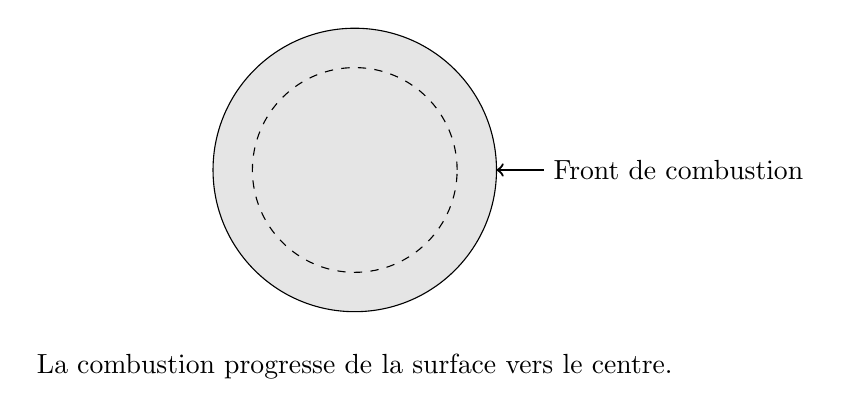
\begin{tikzpicture}

\draw[fill=gray!20] (0,0) circle (1.8);

\draw[dashed]
(0,0) circle (1.3);

\draw[->,thick]
(2.4,0)
--(1.8,0);

\node[right] at (2.4,0)
{Front de combustion};

\node at (0,-2.5)
{La combustion progresse de la surface vers le centre.};

\end{tikzpicture}

\caption{Combustion simplifiée d'un grain sphérique.}
\label{fig:combustion_grain}

\end{figure}

\section{Propagation de la combustion}

Les premiers grains enflammés produisent eux-mêmes des gaz chauds qui
contribuent à enflammer les grains voisins.

La combustion se propage ainsi progressivement à l'ensemble de la charge
propulsive.

Pendant cette phase, la pression dans l'étui augmente rapidement.

\begin{figure}[htbp]
\centering

\begin{tikzpicture}

\foreach \x in {0,...,7}
{
    \fill[gray!30] (\x*0.8,0) circle (0.18);
}

\fill[Part6Color!70]
(0,0) circle (0.18);

\draw[->,thick]
(0.1,0.28)--(0.7,0.28);

\draw[->,thick]
(0.9,0.28)--(1.5,0.28);

\draw[->,thick]
(1.7,0.28)--(2.3,0.28);

\node at (3.0,-0.7)
{Propagation de la combustion};

\end{tikzpicture}

\caption{Propagation simplifiée de l'inflammation entre les grains.}
\label{fig:propagation_combustion}

\end{figure}

\section{Production des gaz}

La combustion transforme une partie de la matière solide en gaz à haute
température.

Ces gaz occupent un volume beaucoup plus important que la poudre initiale.

Comme ils sont confinés dans l'étui et la chambre, leur pression augmente très
rapidement.

\begin{figure}[htbp]
\centering

\begin{tikzpicture}[>=latex]

\draw[thick]
(0,0)
rectangle
(9,3);

\fill[gray!20]
(0.5,0.5)
rectangle
(3,2.5);

\node at (1.75,1.5)
{Poudre};

\draw[->,very thick]
(3.3,1.5)
--
(5.3,1.5);

\fill[Part6Color!20]
(6,0.4)
rectangle
(8.5,2.6);

\node at (7.25,1.5)
{Gaz chauds};

\end{tikzpicture}

\caption{Transformation simplifiée de la poudre en gaz de combustion.}
\label{fig:production_gaz}

\end{figure}

\section{Influence de la géométrie des grains}

La forme des grains joue un rôle essentiel dans le comportement de la poudre.

Selon leur géométrie, la surface disponible pour la combustion peut :

\begin{itemize}
    \item diminuer au cours du temps ;
    \item rester sensiblement constante ;
    \item augmenter progressivement.
\end{itemize}

Cette évolution influence directement la vitesse de production des gaz.

\section{Poudres régressives, neutres et progressives}

Une poudre est dite :

\begin{itemize}
    \item régressive lorsque sa surface de combustion diminue ;
    \item neutre lorsque cette surface reste sensiblement constante ;
    \item progressive lorsqu'elle augmente au cours de la combustion.
\end{itemize}

Le choix dépend du comportement balistique recherché.

\begin{figure}[htbp]
\centering

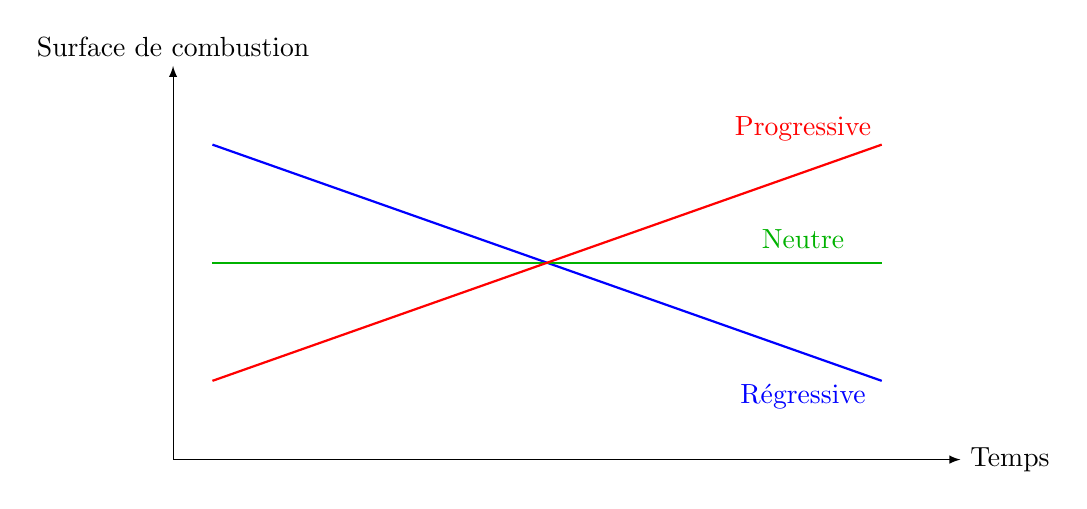
\begin{tikzpicture}[>=latex]

\draw[->] (0,0)--(10,0)
node[right]{Temps};

\draw[->] (0,0)--(0,5)
node[above]{Surface de combustion};

\draw[blue,thick]
(0.5,4)--(9,1);

\draw[green!70!black,thick]
(0.5,2.5)--(9,2.5);

\draw[red,thick]
(0.5,1)--(9,4);

\node[blue] at (8,0.8){Régressive};
\node[green!70!black] at (8,2.8){Neutre};
\node[red] at (8,4.2){Progressive};

\end{tikzpicture}

\caption{Évolution qualitative de la surface de combustion.}
\label{fig:surface_combustion}

\end{figure}

\section{Influence de la pression}

La vitesse de combustion dépend notamment de la pression régnant dans la
chambre.

Lorsque la pression augmente, la combustion tend à s'accélérer.

Il s'établit ainsi une interaction permanente entre la combustion et la montée
en pression.

\section{Influence de la température}

La température de la poudre ainsi que les conditions extérieures peuvent
également influencer la vitesse de combustion.

Ces effets restent généralement limités dans les conditions normales
d'utilisation, mais deviennent importants dans certains domaines comme les
munitions militaires ou spatiales.

\section{Fin de la combustion}

Dans la majorité des cartouches modernes, la plus grande partie de la poudre est
consommée avant que le projectile ne quitte le canon.

Selon la longueur du canon et les caractéristiques de la munition, il peut
néanmoins subsister une faible quantité de poudre imbrûlée.

\section{Combustion et simulation}

\begin{simulation}

Les simulateurs de balistique intérieure ne reproduisent généralement pas la
combustion grain par grain.

Ils utilisent des modèles simplifiés permettant de calculer la vitesse de
production des gaz en fonction des caractéristiques de la poudre, de la pression
et du temps.

Ces modèles offrent un bon compromis entre réalisme physique et coût de calcul.

\end{simulation}

\begin{figure}[htbp]
\centering

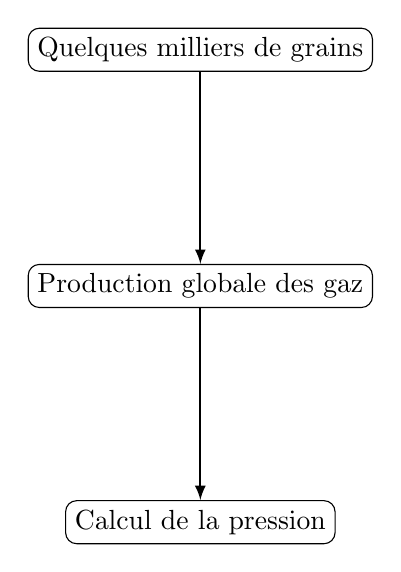
\begin{tikzpicture}[>=latex]

\node[draw,rounded corners]
(A)
at (0,0)
{Quelques milliers de grains};

\node[draw,rounded corners]
(B)
at (0,-3)
{Production globale des gaz};

\node[draw,rounded corners]
(C)
at (0,-6)
{Calcul de la pression};

\draw[->,thick]
(A)--(B);

\draw[->,thick]
(B)--(C);

\end{tikzpicture}

\caption{Principe de simplification utilisé dans les modèles numériques.}
\label{fig:simulation_combustion}

\end{figure}

\section{Vers la montée en pression}

La combustion de la poudre entraîne une production croissante de gaz.

Le chapitre suivant montrera comment cette production de gaz provoque
l'augmentation de la pression dans la chambre, puis la mise en mouvement du
projectile.

\section{À retenir}

\begin{aretenir}

\begin{itemize}
    \item La poudre propulsive brûle par déflagration.
    \item La combustion progresse depuis la surface des grains.
    \item La géométrie des grains influence la production des gaz.
    \item La pression et la combustion s'influencent mutuellement.
    \item La combustion est généralement presque achevée avant la sortie du projectile.
\end{itemize}

\end{aretenir}
